\documentclass[11pt,a4paper,titlepage]{article}

    \setlength{\oddsidemargin}{0in}
    \setlength{\evensidemargin}{0in}
    \setlength{\textwidth}{170mm}
    \setlength{\topmargin}{-15mm}
    \setlength{\textheight}{240mm}
    
    
    \usepackage{hyperref}
    \usepackage{listings}
    \usepackage{graphicx}
    \usepackage{float}
    \graphicspath{ {images/} }
    
    \title{CS26020: Hybrid Controller Report}
    \author{Nathan Williams - naw21}     
    \date{\today}
    
    \begin{document}
    \maketitle
    \tableofcontents
    \listoffigures
    \section{INTRODUCTION}
        This document describes the design, internal model and issues I came across while writing the Hybrid Controller. 
        I completed the whole task of navigating and mapping the maze. 
        I also completed the bonus parts to navigate the robot back to the nest and streaming the maze building over a Bluetooth serial connection to a custom built serial terminal in Java.
        For this assignment I used the Formula allcode robot \cite{Formula all-code} and an in-robot API\cite{in-robot api}, I also used a couple of C standard libraries.
    \section{DESIGN}
        \subsection{State Machine}
            I built my robot around a state machine which I designed before I started writing the code.
            The state machine is split into 3 main parts:
            \begin{itemize}
                \item[Control] This part of the machine looks at the internal model of the robot and controls the next steps that the robot should take.
                \item[Input] This part reads data from the sensors and puts it in the internal model ready for use by the control.
                \item[Output] This part controls the output hardware of the robot, such as the Bluetooth serial, motors, screen and sounds.
            \end{itemize} 
            \begin{figure}[H]
                \caption{State Machine control flow}
                \includegraphics[width=17cm,keepaspectratio]{stateDiagram}
            \end{figure}
        \subsection{Mapping the Maze}
            The Controller maps the maze using a left hand wall following behaviour which works on two levels. 
            The control builds a set of instructions to form a path from the known data in it's internal structure. 
            Once a path is established the instructions are executed in order to get the robot to move from it's current location to its target cell. 
            This is done using reactive behaviours that use the most recent sensor readings from the input step of the state machine.
            Once the robot reaches a new cell the control takes the most recent readings from the sensors and stores them in a map structure. 
        \subsection{Reactive behaviours}
            Most of this task relies on deliberative behaviours but the reactive behaviours caused me the most trouble to code and perfect.
            I begun with two simple functions that turned the robot 90 and drove the robot foreword 15cm.
            \subsubsection{Going foreword 15cm}
                My first problem with the robot going foreword 15cm was that the robot wouldn't do it in a straight line.
                One wheel would always be slightly faster than the other.
                To counter this I took the difference between the left and right encoder values, then increased or decreased the speed of one of the wheels accordingly.
                This ensured that if the wheels got out of sync the speed got adjusted to keep it going in a straight line.
               
                The next issue was that due to the turning 90 degree wasn't perfect the robot would just run itself into the walls and get caught.
                To avoid this I measured the distance the robot was from the walls on it's left and right.
                If the walls were getting too close to the robot, I would decrease the speed of the wheel on the opposite side of the robot which would turn the robot away from the wall.
                
                The combined effect of these two behaviours makes my robot appear to weave as it is going in a straight line, as the two behaviours are fighting.
                This actually was a good combined effect as when the robot approaches a wall it would turn away from it into the wall on the other side. 
                The keeping straight behaviour counters this and straightens the robots path try keep it going straight before it tries to bounce off the next wall.
                This reduces the length of the zig-zag it is doing making the robot move foreword quicker.
            \subsubsection{Turning 90 degree}
                My initial function to turn 90 would only occasional turn a perfect 90 degrees. 
                So to begin I did similar to my going forward method and took the difference between the two encoder values to adjust the speed to keep them moving at the same speed as best I could. 
                
                But it kept over shooting and undershooting the turn. 
                To correct this I used the encoder values to adjust the position of the robot slightly till it is closer to the required encoder tick distance. 
        \subsection{Navigating to the nest}
            While building the maze the robot keeps track of the cell with the lowest light level and holds it in a pointer. 
            Once the maze has been mapped out, the robot will go into the navigate to nest instruction building state. 
            Where it builds a list of instructions using a right hand wall following algorithm with a twist that if checks if the robot will double back on itself.
            If it does it cancels out the instruction and tries a different direction.
            This builds an optimal return route for the robot.
            
            The robot will then leave the route building state and begin executing the instructions until it reaches the stop instruction.
        \subsection{Bluetooth Serial}
            While the robot is navigating the maze I stream data about the robots situation to a custom serial terminal. 
            You can find the source here:

                \url{https://github.com/IdrisTheDragon/Bluetooth-serial-Terminal}

            You will also find a compiled version along with my source and hex file in the code zip file.

            The terminal allowed me to also send detailed debug information from the robot. 
            Which massively helped in debugging and viewing the code while it was running.

            But the main feature is the JavaFx map which updates as I send formatted strings to the terminal allowing a visual representation of the map to be built. 
            Here is a screenshot of the map built by my assessed run of the maze.
            \begin{figure}[H]
                \caption{Assessed run Bluetooth serial terminal output}
                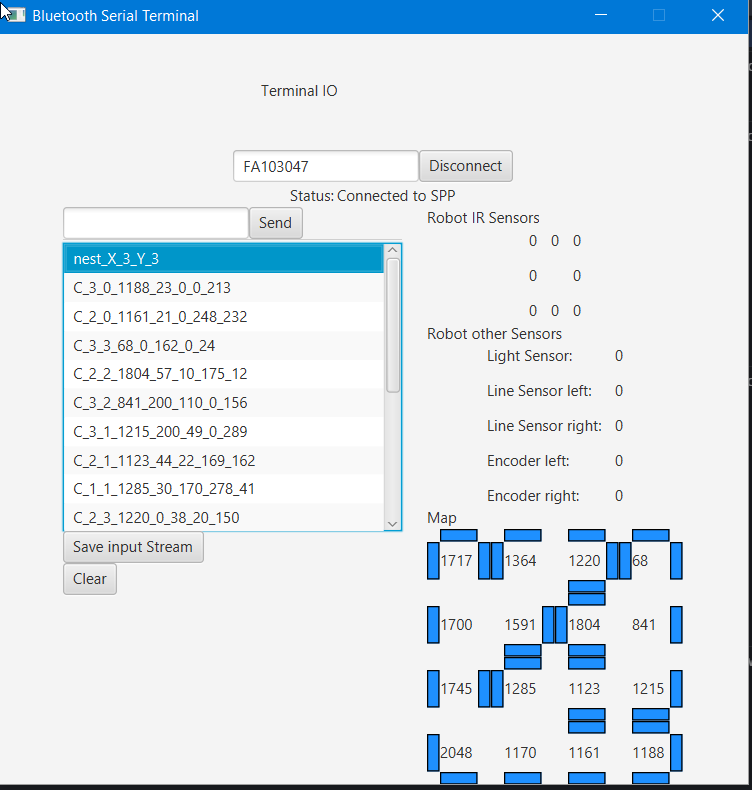
\includegraphics[width=14cm,keepaspectratio]{assessedRun}
            \end{figure}
    \section{INTERNAL MODEL}
        \subsection{Maze}
            The maze is stored in the robot using three structs:
            
            \begin{itemize}
                \item[Cell] The cell struct contains x and y coordinates, pointers to the adjacent walls and an integer to store the light level in that cell.
                \item[HWall] The HWall struct contains pointers to the cells East and West of the potential wall and an integer value that the robot assigns when mapping as to the likely hood that a wall exists here.
                \item[VWall] the VWall struct contains pointers to the cells North and South of the potential wall and and an integer that the robot assigns when mapping as to the likely hood that a wall exists here.
            \end{itemize}

            Upon launch of the robot the maze is built using a couple of for loops linking the cells and walls as appropriate. 
            The outer wall pointer of the cells are filled with NULL values to prevent the robot from leaving the mapping area.
            As the robot maps the maze it navigates the model through the pointers, looking for unexplored cells.
            \begin{figure}[H]
                \caption{Internal model of the maze visualized}
                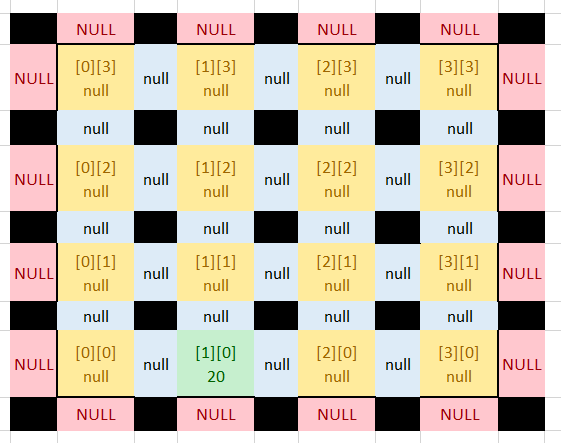
\includegraphics[width=14cm,keepaspectratio]{mazeModel}
            \end{figure}
        \subsection{Environment State(robotState)}
            The information about the robots current state and environment is stored in the robotState struct.
            It contains data about it's current speed, the encoder values, LDR and Infrared sensor values.
            It also contains non environment data such as:
            \begin{itemize}
                \item[orientation] When the robot begins it starts with the arbitrary orientation of North and as the robot turns around the maze, the orientation it is facing changes.
                \item[cellsVisited] As the robot explores the maze it counts the number of cells it has explored. It will stop exploring when this value reaches 16
                \item[curCell \& nest] The robot stores pointers to the cell it is currently in and a pointer to the cell that it thinks is the nest.
                \item[instruction] When a route is plotted the robot stores a linked list of instruction structs with pointers to functions waiting to execute as part of the state machine.
                \item[next] This is a key part of the state machine, as the controller decides the next bit of the state machine the robot should run, this pointer is updated.
            \end{itemize}
    \section{ISSUES AND PROBLEMS}
            \subsection{Reactive Behaviours}
                When moving or turning the robot set distances the robot would frequently over shoot or not go far enough which caused major problems.
                To tackle this I needed to implement reactive behaviours that read the sensors data and help keep the robot straight and turning as accurately as possible.
            \subsection{Deliberative Behaviours}
                Although most of this task relied on deliberative behaviours I didn't really come across any problems while coding this part. 
                Due to using malloc(), calloc() and free() to assign memory I had the occasional memory leak, but they were easy to solve, double checking I was freeing any memory I was allocating.
    \section{FURTURE IMPROVEMENTS}
            \subsection{Reactive behaviours}
                The current Controller uses the bear minimum of reactive control to move the robot, I think I could improve this massively. 

                During the assessed run the robot ran into the corner of a wall and got a wheel caught. 
                Because of this I had to step in and put it back on track so it could continue the run. 
                Adding some check to see if the wheels are caught would help solve this.
                I would code the robot to back up turn slightly before continuing it's course.
            \subsection{Deliberative behaviours}
                With the implementation of navigating to the nest I have used. 
                I would like to adapt the code so it is more general, so it would navigate to a destination. 
                Then once the robot has navigated the maze, I could write a simple function that allows the robot to receive a Bluetooth command and sets the destination cell and the robot could navigate to it.
    
    \clearpage
    \addcontentsline{toc}{section}{REFERENCES}
    \begin{thebibliography}{5}
        \bibitem{Formula all-code} \emph{Formula AllCode Robot}
            \url{https://www.matrixtsl.com/allcode/formula/}
        \bibitem{in-robot api} \emph{in-robot API}
            allcode\_api.h \& allcode\_api.o
            Pete Todd \& Laurence Tyler 1.1
    \end{thebibliography}
    \clearpage

    \label{thelastpage}
\end{document}